\subsection{环 W(A) 的滤子与拓扑}

引理 4．——设 A 为一个环，\(m \geqslant 1\) 为整数。则有

\[
\boldsymbol {a} = \left(a _ {0}, \dots , a _ {m - 1}, 0, \dots\right) + \underbrace {\left(0 , \dots , 0 , \right.} _ {m \text { terms }}, a _ {m}, a _ {m + 1}, \dots)\tag{34}
\]

对 W(A) 中的所有 a 均成立。

设 \(\rho: B \to A\) 为一个满足第 4 节引理 3 条件的环同态。于是 \(W(\rho): W(B) \to W(A)\) 是一个满射环同态，而 \(\Phi_B: W(B) \to B^N\) 是一个单射同态。因此，只需证明有

\[
\Phi_ {n} (\boldsymbol {b}) = \Phi_ {n} (b _ {0},..., b _ {m - 1}, 0,...) + \Phi_ {n} (0,..., 0, b _ {m}, b _ {m + 1},...) \tag{35}
\]

对于 W(B) 中的所有 b 以及所有整数 \(m \geqslant 1, n \geqslant 0\)，均成立。现在有

\[
\begin{array}{r l} \Phi_ {n} (b _ {0},..., b _ {m - 1},... \dots) & = \Phi_ {n} (b _ {0},..., b _ {n}) \quad \text { if } \quad 0 \leqslant n <   m \\ & = \sum_ {i = 0} ^ {m - 1} p ^ {i}. b _ {i} ^ {p ^ {n - i}} \quad \text { if } \quad m \leqslant n \end{array}
\]

\[
\begin{array}{r l} \Phi_ {n} (0, \dots , 0, b _ {m}, b _ {m + 1}, \dots) & = 0 \\ & = \sum_ {i = m} ^ {n} p ^ {i}. b _ {i} ^ {p ^ {n - i}} \end{array} \quad \text { if } \quad 0 \leqslant n <   m \quad \text { if } \quad m \leqslant n,
\]

从而得到公式 (35)。

设 A 为一个环。对于每个整数 \(m \geqslant 0\)，记 \(\mathbf{V}_{m}(\mathbf{A})\) 为 Witt 向量 \(\boldsymbol{a} = (a_{n})_{n \in \mathbb{N}}\) 所成的集合，其中 \(a_{n} = 0\) 对 \(0 \leqslant n < m\) 成立。它是 \(m\) 次幂 \(\mathbf{V}^{m}\)（由映射 \(\mathbf{V}_{\mathrm{A}}\) 得到）的像。公式

\begin{enumerate}
\def\labelenumi{(\arabic{enumi})}
\setcounter{enumi}{35}
\tightlist
\item
\end{enumerate}

\[
\mathrm{V} ^ {m} (\boldsymbol {a} + \boldsymbol {b}) = \mathrm{V} ^ {m} (\boldsymbol {a}) + \mathrm{V} ^ {m} (\boldsymbol {b})\tag{37}
\]

\[
\mathrm{V} ^ {m} (a) \times b = \mathrm{V} ^ {m} (a \times \mathrm{F} ^ {m} (b))
\]

由第 5 节命题 3 对 m 归纳得到。它们蕴含 V \(_{m}\) (A) 是 W(A) 的理想。

\pandocbounded{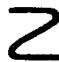
\includegraphics[keepaspectratio]{images/part001_18cee607.jpg}}

置 \(\mathrm{V}_{m}(\mathrm{A}) = \mathrm{W}(\mathrm{A})\)，当 \(m < 0\) 时。序列 \((\mathrm{V}_{m}(\mathrm{A}))_{m \in \mathbf{Z}}\) 是环 \(\mathrm{W}(\mathrm{A})\) 的加法群上的降滤子。它与 \(\mathrm{W}(\mathrm{A})\) 的环结构相容（III，第 2 节第 1 号定义 2）当且仅当 A 是特征为 \(p\) 的环（参见第 3 节例 2 及下文第 8 节命题 5 的推论）。

下文在 W(A) 上赋予拓扑 \(\mathcal{G}\)，它与滤子 \((\mathrm{V}_m(\mathrm{A}))_{m\in \mathbf{Z}}\) 关联。由于 \(\mathrm{V}_m(\mathrm{A})\) 对所有 \(m\in \mathbf{Z}\) 都是 W(A) 的理想，拓扑 \(\mathcal{G}\) 与 W(A) 的环结构相容（TG，III，第 49 页，例 3）。设 \(a\in \mathrm{W(A)}\)；集合 \(a + \mathrm{V}_m(\mathrm{A})\)，其中 \(m\) 遍历 N，构成 \(a\) 关于 \(\mathcal{G}\) 的邻域基。由引理 4 可知，\(a + \mathrm{V}_m(\mathrm{A})\) 由 Witt 向量 \(b\) 组成，并满足 \(a_i = b_i\)（\(0\leqslant i < m\)）。因此，\(\mathcal{G}\) 正是 \(\mathbf{A}^{\mathbf{N}}\) 上各因子离散拓扑的乘积拓扑，故 W(A) 是一个 Hausdorff 且完备的拓扑环（TG，II，第 17 页，命题 10，以及 TG，III，第 22 页，命题 4）。

记 \(\tau_{\mathbf{A}}\)（或简记为 \(\tau\)）为从 A 到 W(A) 的映射，它把 \((a, 0, 0, \ldots)\) 与 A 的每个元素 \(a\) 关联起来。我们有 \(\Phi_n(\tau(a)) = a^{p^n}\)，对每个 \(n \in \mathbb{N}\) 均成立。对任意环同态 \(\rho: \mathbf{B} \to \mathbf{A}\)，都有 W( \(\rho\) ) \(\circ\) \(\tau_{\mathbf{B}} = \tau_{\mathbf{A}} \circ \rho\)。

命题 4．——设 \(a\) 和 \(b\) 属于 \(\mathbf{A}\)，且 \(\boldsymbol{x} = (x_n)_{n \in \mathbb{N}}\) 是 \(\mathbf{W}(\mathbf{A})\) 的一个元素。

\begin{enumerate}
\def\labelenumi{\alph{enumi})}
\tightlist
\item
  有如下公式
\end{enumerate}

\begin{enumerate}
\def\labelenumi{(\arabic{enumi})}
\setcounter{enumi}{37}
\tightlist
\item
\end{enumerate}

\[
\tau (a b) = \tau (a) \times \tau (b)\tag{39}
\]

\[
\tau (a) \times x = (a ^ {p ^ {n}} x _ {n}) _ {n \in \mathbf {N}}.
\]

\begin{enumerate}
\def\labelenumi{\alph{enumi})}
\setcounter{enumi}{1}
\tightlist
\item
  通项为 \(\mathbf{V}^{n}(\tau(x_{n}))\) 的级数在 \(\mathbf{W}(\mathbf{A})\) 中收敛，且其和为 \(x\)。
\end{enumerate}

设 \(n\) 为正整数。第 3 节引入的多项式 \(\mathbf{P}_{n}(\mathbf{X}_{0},\ldots,\mathbf{X}_{n};\mathbf{Y}_{0},\ldots,\mathbf{Y}_{n})\) 是权为 \(p^{n}\) 的关于族 \((\mathbf{X}_{0},\ldots,\mathbf{X}_{n})\) 的等压多项式，其中赋予 \(\mathbf{X}_{i}\) 权 \(p^{i}\)。因此有

\[
\mathrm{P} _ {n} \left(\mathrm{X} _ {0}, 0, \dots , 0; \mathrm{Y} _ {0}, \dots , \mathrm{Y} _ {n}\right) = \mathrm{X} _ {0} ^ {p ^ {n}} \mathrm{P} _ {n} (1, 0, \dots , 0; \mathrm{Y} _ {0}, \dots , \mathrm{Y} _ {n}).\tag{40}
\]

由于 1 = (1, 0, 0, \ldots) 是系数环为 \(\mathbf{Z}[(X_n)_{n\in\mathbb{N}}, (Y_n)_{n\in\mathbb{N}}]\) 的 Witt 向量环的单位元，所以有

\[
\mathrm{P} _ {n} (1, 0,..., 0; \mathrm{Y} _ {0},..., \mathrm{Y} _ {n}) = \mathrm{Y} _ {n}.\tag{41}
\]

以 \(a\) 代替 \(\mathbf{X}_{0}\)，以 \(x_{i}\) 代替 \(\mathbf{Y}_{i}\)，由 (40)、(41) 得到关系式：

\[
\mathrm{P} _ {n} (a, 0, \dots , 0; x _ {0}, \dots , x _ {n}) = a ^ {p ^ {n}} x _ {n}.
\]

根据 W(A) 中乘法的定义，(39) 得证；公式 (38) 是 (39) 的特例。

证明 \(b\)。按定义，\(\mathbf{V}^{n}(\tau(x_{n}))\) 是一个所有分量均为零、但下标为 \(n\) 的分量等于 \(x_{n}\) 的序列。由引理 4 对 \(m\) 归纳可得

\[
\sum_ {n = 0} ^ {m} \mathrm{V} ^ {n} (\tau (x _ {n})) = (x _ {0},..., x _ {m}, 0, 0,...)
\]

对每个整数 \(m \geqslant 0\) 均成立；取极限即得 \(b\)，因为 W(A) 上的拓扑 \(\mathcal{C}\) 是各因子 A 的离散拓扑的乘积。

